%\documentclass[ngerman,dvips]{wkcms}  % latex + dvips
\documentclass[ngerman,pdf]{wkcms}    % pdflatex

\usepackage[utf8]{inputenc}

\title{SSH - The Secure Shell}
\subtitle{Überblick, Technologie, Anwendungsbeispiele}
\author{Susanne Kießling}
\date{\todaylong}

\address
{Hochschule Augsburg\\
 Masterstudiengang Informatik\\
 E-Mail: \url{susanne.kiessling@hs-augsburg.de}      
}

\begin{abstract}
Dfsjkhc sdjfh sdjlkfh sdljkf hlasdjkf haljksdfh asdjlfh als. asdfjk asdjflkha
sdfljhas dfljashd fljkasdhf jlaksdfh lajskdfh alsjkdfh asldjkf hasldjkfh
asljkdfh asljkdf hasljdkfh asljkdfh asljkdfh asljkdfh asljkdfh asljkdfh
asljkdfh alsjkdfh asljkdfh asljkdfh asljkdfh asljkdfh asldkjfh asldkjfh
aslkdjfh.

Asljkdfh alsjkdfh asljkdfh asljkdfh asljkdfh asljkdfh asldkjfh asldkjfh
asljkdfh alsjkdfh asljkdfh asljkdfh asljkdfh asljkdfh asldkjfh asldkjfh
asljkdfh alsjkdfh asljkdfh asljkdfh asljkdfh asljkdfh asldkjfh asldkjfh
aslkdjfh.
\end{abstract}

\keywords{SSH, OpenSSH, Verschlüsselung, TCP/IP-Protokoll}
\categories{Allgemein}

\begin{document}

\maketitle


\section{Einleitung}

Die Übertragung von Daten innerhalb von Computernetzwerken geschieht ohne
entsprechende Vorkehrungen grundsätzlich ungesichert. E-Mails, Passwörter und sämtliche Daten, die übertragen werden, können abgefangen und gelesen werden. SSH (Secure Shell) ist ein Protokoll, das die verschlüsselte Übertragung von Daten über ein Netzwerk ermöglicht \cite{SSH}.
Trotz zahlreicher Berichterstattung über die Folgen von sorglosem Umgang mit Daten in Computernetzwerken, wozu natürlich auch das World Wide Web gehört, ändern viele Nutzer
ihr Verhalten diesbezüglich nicht. Die Sicherheit von privaten Daten ist ein hochaktuelles Thema. SSH (als Protokoll) und dessen Implementierungen stellen eine Möglichkeit dar, Daten innerhalb eines Computernetzwerks sicher zu übertragen. Ziel ist es nun, einen Überblick zu SSH zu geben. OpenSSH dient anschließend als Beispiel-Implementierung, anhand derer die Funktionalitäten gezeigt werden. Der Ablauf eines Verbindungsaufbaus und die verwendeten Verschlüsselungsalgorithmen werden erläutert. Auf aktuelle sicherheitskritische BUGs wird eingegangen. Zur Abgrenzung zwischen der Bezeichnung von SSH als Protokoll bzw. als Implementierung, wird an dieser Stelle festgelegt, dass \IT{SSH} das Protokoll bezeichnet und die Implementierungen explizit benannt werden (bsp. \IT{OpenSSH}).

--> Bereits 19.. entwickelt, in zahlreichen Produkten implementiert
--> Vorgänger telnet, rsh, alles ungesichert

--> evtl. als aktuell erwähnen, dass es auch SSH für mobile Betriebssysteme gibt

 schlechte Passwörter/Bruce Schneier?

SSH (Secure Shell) ist eine unixoide Tralalala...

--> Paper konzentriert sich auf SSH unter Linux
--> Paper will Idee verbreiten, dass mit unscheinbarem Tool einiges möglich ist; ssh wird in vielen Anwendungen verwendet etc.



\newpage

\section{Grundlegendes zu SSH}


SSH verschlüsselt die forlaufende Verbindung zwischen Computern in einem Netzwerk. Dazu verwendet SSH eine Client/Server-Architektur. Abbildung \ref{fig:abb1} veranschaulicht das Grundprinzip von SSH, das laut seiner Spezifikation die Authentifizierung, die Verschlüsselung und die Integrität von Daten, die in einem Netzwerk übertragen werden, beinhaltet.

\begin{figure}[!h] 
\centering 
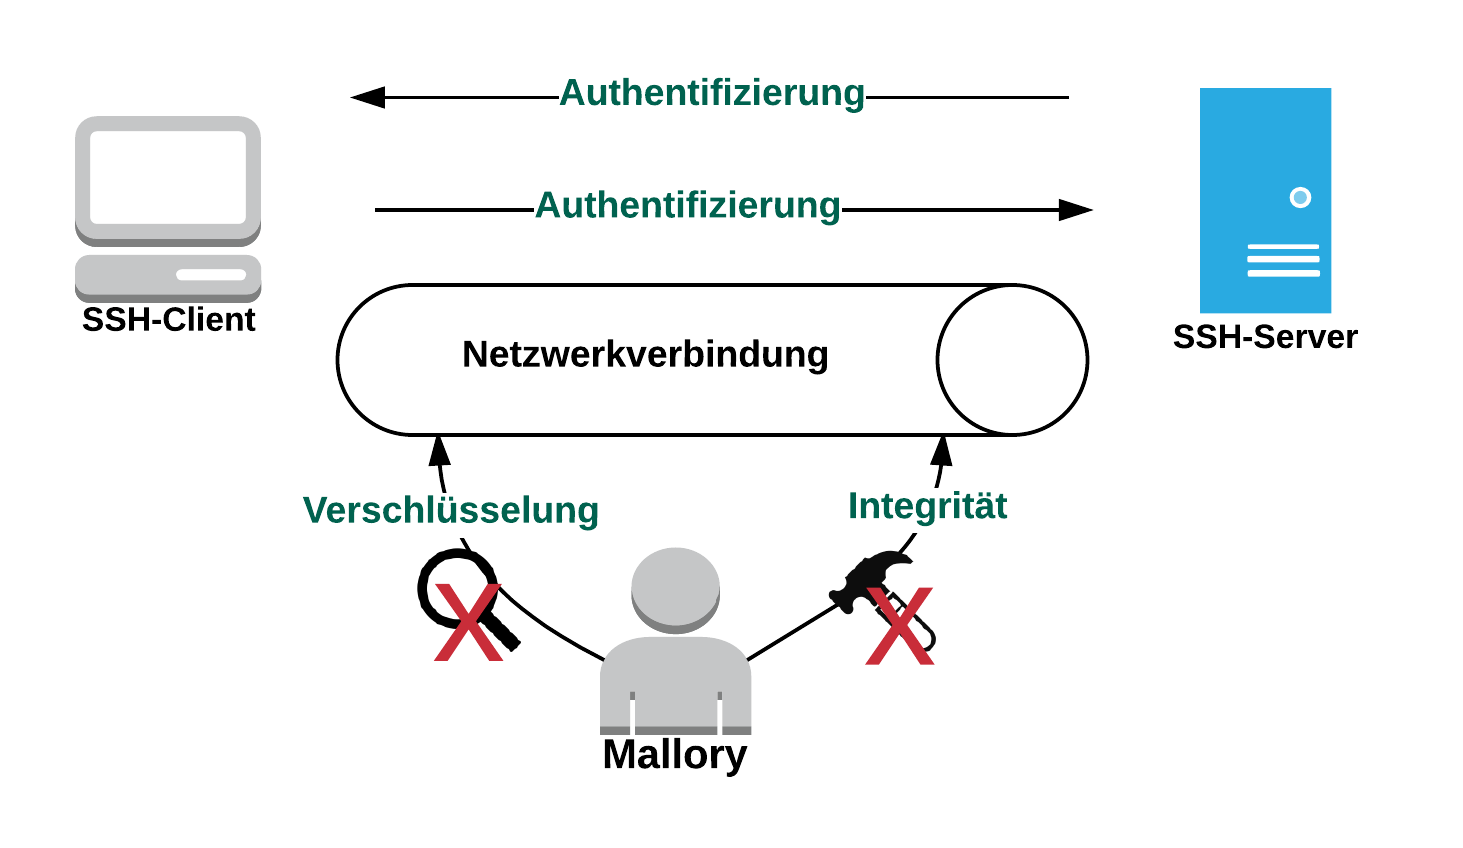
\includegraphics[scale=0.25]{./images/grundprinzip.png}
\label{fig:abb1} 
\caption[Abbildung 1]{Grundprinzip von SSH, eigene Darstellung.} 
\end{figure}
 
Wie in der Abbildung \ref{fig:abb1} zu sehen ist, verlangt eine SSH-Verbindung zwei Authentifizierungen \cite[S. 47]{SSH}. Der Server authentifiziert sich beim Client und umgekehrt (näheres zum Ablauf unter \ref{sec:ablauf}). Zum Verschlüsseln der Daten werden zufällige Sitzungsschlüssel ausgehandelt. Nach Beenden der Sitzung verlieren diese Schlüssel ihre Gültigkeit. SSH garantiert die Integrität der übertragenen Daten, \Dh die Daten können nicht durch einen Dritten (Mallory) verändert werden. 


\subsection{Protokolle}

Das SSH-Protokoll existiert in zwei unterschiedlichen Versionen (SSH-1.x und SSH-2.x), die nicht kompatibel sind. SSH-1 wurde 1995 von Tatu Ylönen an der University of Technology in Helsinki entwickelt. Da es Mängel in der Integritätsprüfung aufweist, ist von einer weiteren Verwendung des SSH-1 Protokolls dringend abzuraten.

SSH-2 ist modular aufgebaut. Die Architektur besteht aus drei Hauptkomponenten: Die Transportschicht, die Authentifizierungsschicht und die Verbindungsschicht. Beschrieben sind die Komponenten durch die \IT{Request for Comments} 4250 bis 4254 der IETF (Internet Engineering Task Force) \cite{ietf}. Ziel der Entwicklung von SSH-2 war es, die Sicherheitsmängel von SSH-1 zu beheben. Außerdem sind weitere Funktionalitäten hinzugekommen. --> evtl. Funktionalitäten aufführen


\subsection{Implementierungen}

Als erste Implementierung des SSH-Protokolls gilt das von Tatu Ylönen 1995 veröffentlichte SSH1.
Es wurde als freie Software veröffentlicht \cite[S. 11]{SSH}. Die Implementierung des SSH-2-Protokolls war hingegen ein kommerzielles Produkt. Die kostenlose Nutzung war nur für Bildungseinrichtungen und den nicht-gewerblichen Bereich erlaubt \cite[S. 22]{SSH}. Folglich kam weiterhin vielerorts die Implementierung des SSH-1-Protokolls zum Einsatz. 1999 entstand das OpenSSH-Projekt, das auf die letzte frei verfügbare Version von SSH aufbaut \cite{OpenSSH}.

Aktuell gibt es verschiedene Implementierungen des SSH-Protokolls. Je nach Einsatzzweck (mobiles Gerät/Workstation) oder Betriebssystem gibt es verschiedene Alternativen. Im Folgenden ist eine kleine Auswahl von Implementierungen mit Kurzbeschreibung aufgeführt.

\subparagraph{PuTTY} steht unter der MIT-Lizenz und stellt einen SSH-Client zur Verfügung. Hauptsächlich wird es unter Windows verwendet, ist aber auch für UNIX-Systeme verfügbar.\cite{putty}  --> Buch ProOpenSSH 

\subparagraph{OpenSSH} Server und Client; vorinstalliert auf allen Linux-Systemen, BSD-Lizenz

\subparagraph{Dropbear} ist eine Implementierung des SSH-2-Protokolls und steht unter der MIT-Lizenz \cite{dropbear}. Dropbear ist vorallem für Systeme mit geringer Prozessorleistung und geringer Speicherkapazität interessant. Es ist auf verschiedenen POSIX-basierten Systemen lauffähig. Eine entsprechende Auflistung ist auf der offiziellen Webseite von Dropbear \footnote{https://matt.ucc.asn.au/dropbear/dropbear.html\#platforms} zu finden.

\subparagraph{Mosh} (mobile shell) bietet erweiterte Funktionalitäten, vorallem für mobile Geräte. Beispielsweise wird die Verbindung bei Roaming aufrechterhalten. Mosh ist keine direkte Implementierung des SSH-Protokolls. Es überträgt keinen Byte-String zwischen Client und Server. Vielmehr tauschen Client und Server einen Snapshot des aktuellen Bildschirms aus \cite{mosh}.

\subparagraph{Lsh} ist eine freie Implementierung des SSH-2-Protokolls, lizenziert untere der GNU GPL \cite{lsh}. --> evtl entfernen






\section{OpenSSH}

OpenSSH dient nun dazu, elementare Funktionalitäten von SSH vorzustellen. Der Client wird unter OpenSSH mit \IT ssh und der Server mit \IT sshd bezeichnet. Alle Konfigurationen bezüglich Client und Server sind in den jeweiligen Konfigurationsdateien zu finden (Client: ssh\_config, Server: sshd\_config)


Für alle Funktionalitäten gibt es unter der jeweiligen \IT manpage (Manual Page) eine Übersicht der verfügbaren Optionen (\$ man ssh, \$ man scp, \$ man sshfs, \$man ssh-keygen, \$ man ssh-copy-id). 

\subsection{Remote Terminal Session}

Der enfternte Login auf einem Server ist das Basis-Feature von OpenSSH.
Dazu ist lediglich der Befehl \IT ssh und der \IT hostname, zu dem eine Verbidung aufgebaut werden soll, notwendig. Alle anderen Werte sind optional.
Eine Übersicht der Parameter ist auf den manpages von SSH zu finden
(\$ man ssh).

\begin{program}

[sue@kaktus]\$ ssh micra@login.rz.hs-augsburg.de
micra@login.rz.hs-augsburg.de's password:
%Linux bug 3.2.0-4-amd64 #1 SMP Debian 3.2.65-1+deb7u1 x86_64
Plan your installation, and FAI installs your plan.

Last login: Mon Apr 25 22:38:45 2016
from p5088ff5b.dip0.t-ipconnect.de
micra@bug:~\$
micra@bug:~\/tmp\$ exit
logout
Connection to login.rz.hs-augsburg.de closed.

\end{program}

Im Beispiel loggt sich der Benutzer \IT sue (Client: \IT kaktus) unter dem Benutzer \IT micra auf dem Server \IT login.rz.hs-augsburg.de ein. Anschließend authentifiziert der Server den Client durch eine Passwortabfrage. Mit \IT micra@bug:~\$ steht das Remote-Terminal zur Verfügung. Mit \IT exit kann die Sitzung beendet werden. Neben der Passwortabfrage ist es möglich, sich über einen SSH-Schlüssel beim Server zu authentifizieren.

Bei jedem Sitzungsaufbau wird clientseitig geprüft, ob der öffentliche Schlüssel des Servers in der Liste bereits bekannter Hosts (\IT known\_hosts) enthalten ist. Handelt es sich um den ersten Login auf einem Server, gibt es einen Warnhinweis, dass es keinen Eintrag in der known\_hosts Datei gibt. Dieser Mechanismus soll Man-in-the-Middle Angriffe verhindern. Stimmt der Benutzer dem Fortfahren zu, wird der öffentliche Schlüssel des Servers in die \IT known\_hosts Datei aufgenommen und beim nächsten Sitzungsaufbau kommt es zu keinem erneuten Warnhinweis. \cite[S. 25]{SSH}

--> remote-session wird in vielen Anwendungen verwendet

\subsection{Datenübertragung mit \IT{scp}}

\IT scp steht für \IT secure \IT copy und ermöglicht die gesicherte Übertragung von Daten zwischen Client und Server. Es können einzelne Dateien bis hin zu ganzen Verzeichnisstrukturen kopiert werden. \cite[S. 80]{openssh_book} Mit dem Befehl \IT scp, der Datei, die kopiert werden soll und der Angabe des Zielservers sind alle Pflichtparameter vorhanden. Nach Abfrage des Passworts durch den Server wird der Fortschritt der Datenübertragung angezeigt.

\begin{program}
[sue@kaktus ~]\$ scp hello\_all.txt
micra@login.rz.hs-augsburg.de:~
micra@login.rz.hs-augsburg.de's password:
hello\_all.txt        100\% 6297     6.2KB/s   00:00
\end{program}

Im Beispiel wird die Datei \IT hello\_ \IT all.txt vom Homeverzeichnis des Clients (sue@kaktus) in das Homeverzeichnis des Servers ( micra@login.rz.hs-augsburg.de:~) kopiert. Unter Angabe eines Dateinamens hinter dem Server kann die Datei auf dem Server beliebig benannt werden. In den manpages von sshfs sind noch zahlreiche Optionen zu finden (\$ man sshfs).

Aus dem Beispiel wird deutlich, dass \IT scp eine simple und effiziente Möglichkeit darstellt, Dateien sicher zwischen Client und Server zu übertragen. Es eignet sich beispielsweise hevorragend, um als Systemadministrator Aktualisierungen oder diverse Medien zu verteilen. \cite[S. 80]{openssh_book}

--> reguläre Ausdrücke sind möglich \\
--> rekursiv kopieren
--> 

\subsection{Dateisystem einhängen mit \IT{sshfs}}

Mit \IT sshfs (\IT Secure \IT Shell \IT File \IT System) lassen sich entfernte Verzeichnisse ins lokale System einhängen. Beim Client kommt dafür das FUSE (Filesystem in Userspace) Kernel-Modul zum Einsatz. Der große Vorteil ist hier, dass der Benutzer am Client-PC mit den eingehängten Dateien arbeiten kann, als wären es lokale Dateien.

Zum Einhängen ist der Befehl \IT sshfs, der \IT host und der \IT mountpoint,
\Dh der Pfad an dem das Verzeichnis eingehängt werden soll, notwendig.
Mit dem Befehl \IT unmounting \IT fusermount lässt sich das eingehängte Verzeichnis entfernen.

\begin{program}
sshfs [user@]host:[dir] mountpoint [options]

# Verzeichnis aushängen:
unmounting fusermount -u mountpoint
\end{program}

Als Vorteil gegenüber vergleichbaren Tools, wie NFS oder Samba nennen die Entwickler von \IT sshfs beispielsweise das automatische Einhängen der Verzeichnisse über ein Shell-Skript. Außerdem bietet \IT sshfs den Vorteil, dass Verzeichnisse an beliebiger Stelle eingehängt werden können, unabhängig von zentral verwalteten Tabellen (/etc/fstab), die festgelegte Mount-Verzeichnisse enthält. \cite{sshfs}

\subsection{Schlüssel generieren mit \IT ssh-\IT keygen}

Der Client authentifiziert sich beim Server standardmäßig über die Eingabe eines Passworts. Die Verwendung von Passwörtern bringt jedoch verschiedene Nachteile mit sich. Häufig werden unsichere Passwörter verwendet, die leicht auf Brute-Force-Attacken oder Wörterbuchanalysen ansprechen.\cite{schneier} Außerdem kann das Passwort auf einem unterwanderten Server abgefangen werden, auch wenn die Übertragung selbst gesichert war. \cite[S. 29]{SSH}

Daher bietet OpenSSH \IT Public-Key-Authentifizierung an. Hierzu wird ein Schlüsselpaar bestehend aus einem privaten und einem öffentlichen Schlüssel benötigt. Der private Schlüssel ist geheim, der öffentliche Schlüssel wird auf dem Server hinterlegt. \cite[S. 114]{openssh_book} (näheres hierzu bei Ablauf einer sicheren Verbindung). An dieser Stelle kommt \IT ssh-keygen zum Einsatz. Mit diesem Tool ist es möglich, das Schlüsselpaar unkompliziert und komfortabel erstellen zu lassen. Standardmäßig erzeugt \IT ssh-keygen ein RSA-Schlüsselpaar. Andere Verschlüsselungsverfahren können durch Optionen ausgewählt werden (welche sind das genau?). --> evtl. Referenz Buch, PublicKeyAuth

--> Schlüssellänge

\begin{program}
[sue@kaktus ~]\$ ssh-keygen
\end{program}

--> es kann ein Passwort vergeben werden, um ssh-Schlüssel zu sichern


Nach dem Erstellen der Schlüssel legt \IT ssh-keygen das lokale Verzeichnis \IT .ssh an. Dort wird der öffentliche und private Schlüssel gespeichert.

Im nächsten Schritt muss der öffentliche Schlüssel auf dem Server hinterlegt werden. Dazu stehen verschiedene Möglichkeiten zur Verfügung. Man könnte den öffentlichen Schlüssel mit dem Befehl \IT scp auf den Server kopieren und zwar in das Verzeichnis \IT .ssh\/authorized\_keys. Wesentlich einfacher funktioeniert es mit dem Befehl \IT ssh-copy-id. Unter Angabe des \IT hostname kopiert der Befehl \IT ssh-copy-id den öffentlichen Schlüssel automatisch ins Verzeichnis \IT .ssh\/authorized\_keys des Servers.

\begin{program}
[sue@kaktus ~]\$ ssh-copy-id micra@login.rz.hs-augsburg.de
\end{program}

Um Public-Key-Authentifizierung durchführen zu können, muss es vom Server freigegeben sein. Das Attribut \IT PubKeyAuthentication sollte dafür in der Konfigurationsdatei des Servers auf \IT yes gesetzt sein. \cite [S. 116]{openssh_book}

\subsection{Weitere Funktionalitäten}

\paragraph{SSH-Agenten}
Die Eingabe der Passphrase für die Freigabe des SSH-Schlüssels muss bei jeder Remote-Verbindung neu durchgeführt werden. SSH-Agenten ermöglichen es,
dass die Passphrase lediglich einmal pro Session abgefragt wird. Für alle weiteren Remote-Verbindungen, die aufgebaut werden, speichert der SSH-Agent die privaten Schlüssel. \cite[S. 230]{SSH} \cite[S. 132]{openssh_book}

\paragraph{Forwarding}

SSH macht es möglich, den Datenstrom von TCP/IP-Anwendungen zu verschlüsseln.
Das wird \IT Port-Forwarding, oder auch \IT Tunneling genannt. \cite[S. 337]{SSH} Um Port-Forwarding ausführen zu können, muss TCP-Forwarding in der Konfigurationsdatei des Servers als erlaubt gekennzeichnet sein. \cite[S. 151]{openssh_book}

Mit \IT X-Forwarding kann die entfernte grafische Oberfläche auf dem lokalen Rechner dargestellt werden. 

\paragraph{Konfigurationsdateien}

--> ssh\_config \\
--> sshd\_config \\



\section{Sicherheitsrelevante Betrachtung}


\subsection{Ablauf einer sicheren Verbindung}\label{sec:ablauf}

\paragraph{Verbindungaufbau}
Der Aufbau einer sicheren Verbindung läuft grob wie folgt ab: Der Client sendet eine Anfrage an den Server. SSH nutzt hier standardmäßig Port 22, das ist jedoch konfigurierbar. Der Server gibt seine Identität (host-ID), das verwendete Protokoll (SSH-1, SSH-2) und weitere Daten bekannt. Falls der Client zum ersten Mal mit dem Server kommuniziert, wird eine Warnung ausgegeben. Fährt der Client fort, wird die host-ID in die Liste der \IT known\_hosts aufgenommen. Für die Sitzung wird mittels Diffie-Hellman-Verfahren ein Session-Key erzeugt. Abschließend wählt der Client eine der vorgeschlagenen symmetrischen Verschlüsselungsverahren --> angeben, welche zur Auswahl stehen bei SSH

\paragraph{Authentifizierung}
An dieser Stelle ist die Verbindung verschlüsselt und die Authentifizierung findet statt. Für eine Public-Key-Authentifizierung sieht dies folgendermaßen aus: Der Server generiert einen Zufalls-String und verschlüsselt diesen mit dem öffentlichen Schlüssel des Clients. Der Client entschlüsselt diesen Zufalls-String mit seinem privatem Schlüssel. Anschließend kombiniert der Client den entschlüsselten String mit dem Session-Key und generiert daraus eine md5-Hashsumme. Der Server führt diese Aktion ebenfalls durch und vergleicht die beiden md5-Hashsummen. Stimmen die beiden Summen überein, ist der Client erfolgreich authentifiziert. \cite[S. 64]{SSH} \cite{man_ssh}




\subsection{Aktuelle/Bekannte Schwachstellen}
Sicherheitskritische BUGs häufig nicht direkt in SSH, sondern in Komponenten, auf die SSH aufbaut, z.B. OpenSSL.

http://www.openssh.com/security.html

\subsection{Anforderungen an den Serveradministrator}

Der Administrator eines SSH-Servers muss grundsätzlich dafür sorgen, dass die verwendete Software aktuell ist. Die Konfigurationsdatei enthält Standardwerte und muss auf den jeweiligen Anwendungsfall angepasst werden.
Der Zugriff auf die Konfigurationsdatei ist nur mit Root-Rechten möglich.
Handelt es sich um ein sehr sicherheitskritisches System, könnte man eine Prüfsumme (md5, SHA1) der Konfigurationsdatei erstellen, um mögliche Manipulationen zu erkennen. \cite[S. 50]{openssh_book}

Empfehlenswerte Änderungen/Einstellungen der Konfiguration:

\IT PermitEmptyPasswords no: Diese Option muss zwingend auf \IT no gesetzt sein. Andererseits ist es möglich, dass sich Clients ohne Passwort einloggen können.

\IT RhostsAuthentication no, RhostsRSAAuthentication no, IgnoreRhosts yes, IgnoreRootRhosts yes: 








\newpage


\section{Fazit \& Ausblick}
--> sehr simpel und effizient
--> betrachtet man die nicht vorhandene Sensibilität bezüglich sicheren Passwörtern, ssh sinnvoll, bzw. mit ssh-key


\bibliography{sample}
\bibliographystyle{alphadin}
%\bibliographystyle{apalike}

\end{document}


